\documentclass[11pt,a4paper,oldfontcommands]{memoir}
\usepackage[utf8]{inputenc}
\usepackage[T1]{fontenc}
\usepackage{microtype}
\usepackage[dvips]{graphicx}
\usepackage{xcolor}
\usepackage{times}
\usepackage{titlesec}
\usepackage{wrapfig}
\usepackage{float}



\usepackage[
breaklinks=true,colorlinks=true,
%linkcolor=blue,urlcolor=blue,citecolor=blue,% PDF VIEW
linkcolor=black,urlcolor=black,citecolor=black,% PRINT
bookmarks=true,bookmarksopenlevel=2]{hyperref}

\usepackage{geometry}
% PDF VIEW
 \geometry{total={210mm,297mm},
 left=25mm,right=25mm,%
 bindingoffset=0mm, top=25mm,bottom=25mm}
% PRINT
%\geometry{total={210mm,297mm},
%left=20mm,right=20mm,
%bindingoffset=10mm, top=25mm,bottom=25mm}

\OnehalfSpacing
%\linespread{1.3}

%%% CHAPTER'S STYLE
%\chapterstyle{bianchi}
%\chapterstyle{ger}
%\chapterstyle{madsen}
%\chapterstyle{ell}
\titleformat{\chapter}
  {\Large\bfseries} % format
  {}                % label
  {0pt}             % sep
  {\huge}  
%%% STYLE OF SECTIONS, SUBSECTIONS, AND SUBSUBSECTIONS
\setsecheadstyle{\Large\bfseries\sffamily\raggedright}
\setsubsecheadstyle{\large\bfseries\sffamily\raggedright}
\setsubsubsecheadstyle{\bfseries\sffamily\raggedright}


%%% STYLE OF PAGES NUMBERING
%\pagestyle{companion}\nouppercaseheads 
%\pagestyle{headings}
%\pagestyle{Ruled}
\pagestyle{plain}
\makepagestyle{plain}
\makeevenfoot{plain}{}{\thepage}{}
\makeoddfoot{plain}{}{\thepage}{}
\makeevenhead{plain}{}{}{}
\makeoddhead{plain}{}{}{}

\def\code#1{\texttt{#1}}


\maxsecnumdepth{subsection} % chapters, sections, and subsections are numbered
\maxtocdepth{subsection} % chapters, sections, and subsections are in the Table of Contents


%%%---%%%---%%%---%%%---%%%---%%%---%%%---%%%---%%%---%%%---%%%---%%%---%%%

\begin{document}

%%%---%%%---%%%---%%%---%%%---%%%---%%%---%%%---%%%---%%%---%%%---%%%---%%%
%   TITLEPAGE
%
%   due to variety of titlepage schemes it is probably better to make titlepage manually
%
%%%---%%%---%%%---%%%---%%%---%%%---%%%---%%%---%%%---%%%---%%%---%%%---%%%
\thispagestyle{empty}

{%%%
\sffamily
\centering
\Large
~\vspace{\fill}

{\huge 
An Open-Source Event Based SCADA System for the Power Grid
}

\vspace{2.5cm}

{\LARGE
Trevor Aron
}

\vspace{3.5cm}

A project report submitted to the Johns Hopkins University in
conformity with the requirements for the degree of Master 
of Science in Engineering\\ 

\vspace{3.5cm}

Advisors: Dr. Yair Amir, Tom Tantillo

\vspace{\fill}

May 2017

%%%
}%%%

%%%---%%%---%%%---%%%---%%%---%%%---%%%---%%%---%%%---%%%---%%%---%%%---%%%
%%%---%%%---%%%---%%%---%%%---%%%---%%%---%%%---%%%---%%%---%%%---%%%---%%%

\chapter{Acknowledgements}

\indent \indent I would like to thank Marco Platania. Marco Platania really introduced me to
what SCADA actually is. We came up with the scenario that I would end up building
together after scouring the internet for youtube videos of HMI demos. Marco
was also the first person to realize the limitations of PvBrowser and split
the HMI and Data Acquisition portions, leading to the creation of the new SCADA 
architecture I am now presenting. \\

\indent I would like to thank Tom Tantillo. Tom Tantillo really spearheaded turning
this project into the full Spire system, which will be his pHD thesis. He worked
with me tirelessly to get this made. Tom has an amazing ability to get things
done, and done well, no matter how impossible it seems.
He has served as one of my main mentors, helping me with everything from 
writing posters to drafting emails. Much of this
work was on his suggestion. \\

\indent I must also thank Yair Amir. He was my professor in Intermediate Programming, 
Distributed Systems, and Advanced Distributed System. It was he who made me
interested in systems. It was also he who had the vision for intrusion tolerant
SCADA and fortunately invited me to help. I truly admire his desire to
protect the nations infrastructure for the good of society. \\

\indent Finally I would like to thank Amy Babay. Amy Babay has helped me in countless ways
and is always there to answer my questions. She also made significant work towards
Spire .
\clearpage
\tableofcontents*

\clearpage

%%%---%%%---%%%---%%%---%%%---%%%---%%%---%%%---%%%---%%%---%%%---%%%---%%%
%%%---%%%---%%%---%%%---%%%---%%%---%%%---%%%---%%%---%%%---%%%---%%%---%%%

\chapter{Introduction}

\section{Abstract}

\indent \indent This document presents the construction of an open-source event-based SCADA 
architecture. This construction is used as a backbone of the Spire Intrusion Tolerant
SCADA system. The aim of this work is to build a SCADA system that is scalable, and has an 
easy to work with architecture that is still backwards compatible with
SCADA equipment. The key component of this architecture is the RTU/PLC Proxy. This additional 
machine allows the SCADA system to be fully backwards compatible with devices while
making sure that updates from devices are delivered to the core system as changes occur.
Additionally this extra component provides an additional layer of security to the SCADA
system.

\section{Background}

\subsection{SCADA}

\indent \indent SCADA stands for Supervisory Control and Data Acquisition. 
They are systems used 
to monitor and control physical devices in critical infrastructure applications.
Such applications include railways, electrical grids, power generation,
and factorys. ~\cite{SCADA in the Light of Cyber Warfare}. \\

\begin{figure}[ht]
  \begin{center}
  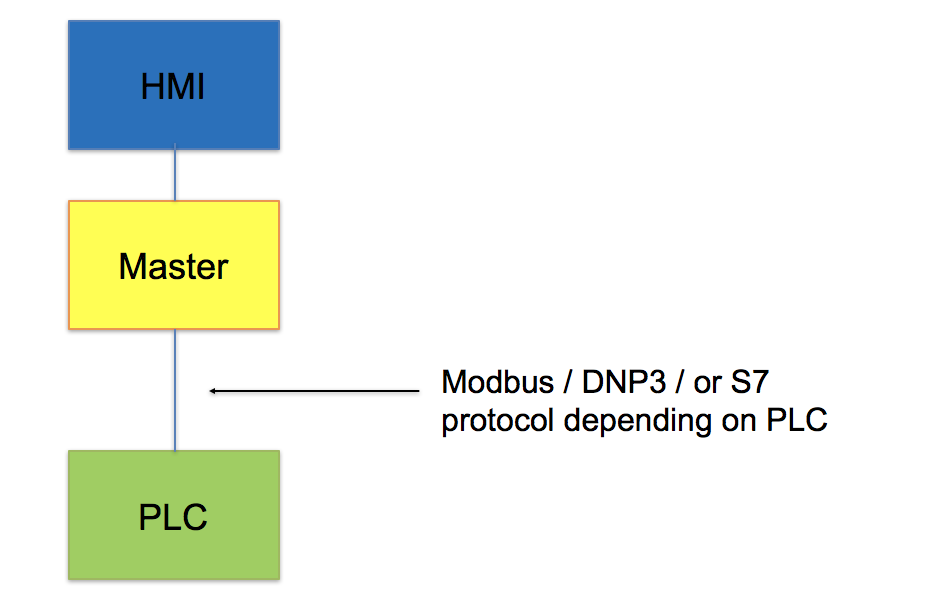
\includegraphics{normal_scada}
  \caption{Architecture of a SCADA System}
  \label{fig:1}
  \end{center}
\end{figure}

SCADA systems are very different depending on the scenario being monitored and control.
These specific conditions can influence the topology of the network and the
protocols being used to communicate between the Master and PLC. \cite{Security issues in SCADA networks} 
They are also
mainly vendor locked, changing wildly depending on what company built the system. However,
all SCADA systems share the basic architecture described in Figure \ref{fig:1}. 
This shows the three main portions of any control system: the Human Machine
Interface (HMI), the SCADA Master, and the Programmable Logic Controller (PLC) or Remote 
Terminal Unit (RTU). \\

The Human Machine Interface is the machine that visualizes the data to a Human operator,
and allows said operator to make changes to the system. What an HMI looks like is very 
specific on the critical infrastructure system being monitored. Usually, they are set
up with images that look like the actual system -- an HMI monitoring water levels may
have an image of a tank with a variable amount of water in it. They can also just be
numbers on a screen -- it really depends on the system and the company making the HMI.\\

Programmable Logic Controllers and Remote Terminal Units are the devices in the
system actually being monitored and controlled. These machines are in the field and will
either be integrated with the devices. RTU's are a little more intelligent
than PLC's and are usually outfitted with advanced communication systems such as radio.
They may also perform some small automated control tasks. They are specifically for 
SCADA systems. PLC's are a bit more generic, and most hobbyist boards (such as Arduino's)
can be considered as a PLC. RTU's and PLC's in SCADA systems are usually vendor 
created, closed source devices. They also communicate with legacy communication protocols, 
which have been around since the seventies and eighties. 
There are many different protocols,
three common ones for power grids are Modbus, DNP3, and Siemens S7. Beyond these protocols,
the American Gas Association's AGA-12 standard states that there are between 150-200
different SCADA communication protocols. \cite{Security issues in SCADA networks} \\

The SCADA Master is the brain of the system. All commands from the HMI first go to the
SCADA Master before they are sent to a PLC. The SCADA Master typically speaks whatever
protocol languages the PLC's and RTU's it monitors can speak. The SCADA Master typically
has automated control and alerting abilities. They also contain a historian which
keeps an audit trail of operational data. \cite{SCADA in the Light of Cyber Warfare}  \\

\section{Motivations}

\indent \indent
There are four main motivations for building this open source
event based architecture.
The first is Security: the RTU Proxy component in the event based SCADA architecture
provides a powerful layer of security. 
The second is scalability: an event based system pushes less
data over the network. The third is for replication: it is much easier to replicate
an event based system than a polling based system. The final is the motivation for
open source: adoption.

\subsection{SCADA Security}

\indent \indent SCADA systems were designed in the earlier days of computing before cyber security was
a real consideration. However, recent evidence shows that SCADA systems need to make
security a priority.\\

Stuxnet is a virus, first identified in 2010, that was discovered to
target Siemens SCADA systems. Specifically, it was aimed at the
Siemens SCADA systems that controlled nuclear enrichment facilities in Iran.
The system was air gapped, but the virus entered by copying itself on
remote drives and spreading in private networks. It affected computers that
were used to modify and program PLC's and used this to insert malitious code
into a PLC that would make it function incorrectly. \\

The onset of Stuxnet lead the world to look carefully at SCADA systems and
their cyber security. The test in \cite{Who is attacking your SCADA Equipment} shows
the extent of the threat. They set up a honey pot of PLC's connected to the internet.
In a month time frame there where over 39 attacks from 14 different countries. 
SCADA systems have traditionally used air gapped networks to create security, but
many of these PLC's and RTU's are configured incorrectly or connected to the
internet such that employees can access and modify them from home. One can
find PLC's on the internet with a basic search. The website Shodan is a 
search engine designed to discover Internet of Things (IOT) devices on the internet.
They have an entire section devoted to finding industrial control equipment by looking for
IP connected devices with common SCADA protocol ports open. \cite{Shodan} \\

The weakest parts of the system are the devices. They are hard to harden:
PLC's may have very limited computational abilities. They also often run on
real time operating systems which are lighter weight, but provide less security. Thus, many
PLC's can not support running a firewall. \cite{Security Issues in SCADA Networks} In
addition, because they run on real time operating systems, they are more susceptible
to disruption from denial of service attacks.
Beyond the PLC itself, the protocols they
speak are not secure. Most typically do not support cryptography primitives.
This is also due to the limited computing power of the devices. Thus most 
communication to the devices is unencrypted and most commands are unauthenticated. For
instance, Modbus is sent over the wire completely unencrypted, with no integrity checks,
and no authentication. If one is on the same networks as a device that speaks Modbus,
they can do whatever they want. \cite{Secure Modbus} In addition, because the
world of SCADA is vendor locked, many of these protocols have been
programmed from scratch for a particular device. Many of these implementations
are not robust and have bugs. In our own experiments with the ASE Test Set 2000
RTU emulation device we found that it had bugs in it's implementation of DNP3. These
bugs are often the entry way for intruders. \\

There have been many efforts to harden PLC's. For instance,  the efforts in this
paper \cite{Secure Modbus} propose a new Modbus protocol that is translated
by a middle gateway device into regular Modbus for backwards compatibility 
with devices. The secure modbus However, this breaks backwards compatibility with masters. A more broad based
 approach has also been to attach  machines at
both ends, one at the SCADA Master, and the other at the RTU or PLC.
\cite{Security Issues in SCADA Networks} This acts as a bump in the wire
in which data is encrypted. To solve the firewall issue, there
has also been efforts to place small firewalls in front of each PLC in a network.
\cite{Security Issues in SCADA Networks} \\

The solution that I propose, the RTU proxy, solves these issues. The RTU Proxy is a 
machine that will be placed in front of RTU's or PLC's on the network. It
translates commands from the Master into the specific PLC or RTU communication 
protocol for the corresponding device. This proxy runs a firewall for the devices
that is speaks to, removing them from direct access to the wide area network. Since
the proxy is a modern machine, and not a device board, it can also preform cryptographic
primitives. Thus, the information it gets from the Master has authentication, integrity,
and confidentiality. Since it speaks many differing SCADA protocols, it provides
backwards compatibility for devices.


\subsection{Scalability}

\indent \indent
There are two different SCADA protocol architectures. The first is a polling model, and
the second is an event based model. An event based model consists of the device only
sending updates to the master whenever there is a change of state. DNP3 is an
event based protocol. The polling
model consists of the master sending requests for updates to the devices
at different polling intervals. Modbus is a polling protocol.\\

\indent
One of the issues with the polling model is that it doesn't scale. Each device
takes a constant amount of bandwidth. This is expensive. Some devices may transmit
a lot of data on each polling interval. There are some SCADA systems, like smart
grids, are very large. There is an estimated 150,000,000 meters installed in Europe.
\cite{Event-based hybrid metering feeding AMI and SCADA}. If the devices only
speak a protocol like Modbus, then there would be a massive amount of bandwidth
used. In addition the historian would have to store much more data. Event based
models are more efficient because only when a device's state has changes they send data.\\

\indent
The need for SCADA scalability has been recognized by others in the field.
SAP and Schneider Electric have laid out their vision for the future in SCADA in the
following paper: \cite{Architecting the next generation of service-based SCADA/DCS system of systems}. 
They address that it is impossible to perform polling in large scale SCADA systems, and
suggest the transition to even driven infrastructures is the future. However, they stress
that future SCADA systems must stay backwards compatible to work with existing devices.
The authors of \cite{Event-based hybrid metering feeding AMI and SCADA} were running
a smart grid monitoring system. In order to scale this monitoring, they created a new 
protocol and communication pattern. The issue with this work, in greater adoption,
is that it breaks backwards compatibility, and new devices need to be made. 
SCADA systems can use DNP3 devices and solve this issue, but not all devices speak
DNP3.\\

\indent
The solution I propose has a device, the RTU proxy, colocated with devices. The RTU
proxy speaks multiple SCADA protocols (currently Modbus and DNP3, but it can be extended
to many more) and translates
this information to a generic format the SCADA master understands. The Proxy
can be designed such that it only pushes information when there is a change in state.
This solution makes all SCADA systems have more homogenous communication patterns despite
the devices that may need to be used.

\subsection{Replication}

\indent \indent
One of the goals of this work was to make SCADA software such that the master could
be replicated. Replication opens the door for making SCADA systems more available:
a system could be replicated with Paxos to be fault tolerant,
or a byzantine fault tolerant algorithm to make the system intrusion tolerant -
allowing it to work even if components have been compromised by an intruder.
Specifically, this system was used to make Spire, an intrusion tolerant SCADA
system. \\

\indent 
A former member of the DSN lab, John Kirsch, published a paper \cite{Survivable SCADA Via
Intrusion-Tolerant Replication}
about his efforts in making a Siemens SCADA system intrusion tolerant. He notes that 
intrusion tolerant replication systems, such as Prime, assume that updates are 
client driven (event based), while some SCADA systems process requests that are
server driven (polling). This mismatch forced him to create the intrusion tolerant timeout
protocol. Not only is this protocol non trivial to implement, it also requires additional
Prime orderings which negatively impact system performance by increasing load. \\

\indent
By making an event based system, this extra intrusion tolerant timeout protocol is no
longer needed, and backwards compatibility is still supported. This makes replication
of the system much simpler, and conserves the number of updates that need to be ordered.\\


\subsection{Adoption}

\indent \indent

Finally, the motivation to build this system entirely with open source components is
to encourage usage and adoption in the SCADA community. The efforts of John Kirsch in
\cite{Survivable SCADA via Intrusion-Tolerant Replication} are unfortunately unavailable
as Siemens decided not to release this product. By building a completely open source
SCADA system, this work can be used as a base for SCADA security research to build off
of. Spire is able to be released as open source because this system is uses all
fully open source parts. \\

\indent 
In addition, using open source components mean that this
system will benefit as the differing parts get further research. OpenDNP3 \cite{OpenDNP3}
is currently maintained by a group that performs vulnerability research on SCADA
protocols. We use this for our DNP3 implementation, and the security of our
system will be improved from their work. We use OpenPLC \cite{OpenPLC} to emulate PLC's 
in this system. This integration benefits our system as Open PLC is being designed to
be used as a vehicle for PLC security research, and when the security of Open PLC improves,
so will our system. In addition Open PLC supports a wide variety of real PLC
boards to deploy on, which may encourage others to adopt this solution.\\

\chapter{Open Source Event-Based Architecture}

\section{Overview}

\begin{figure}[ht]
  \begin{center}
  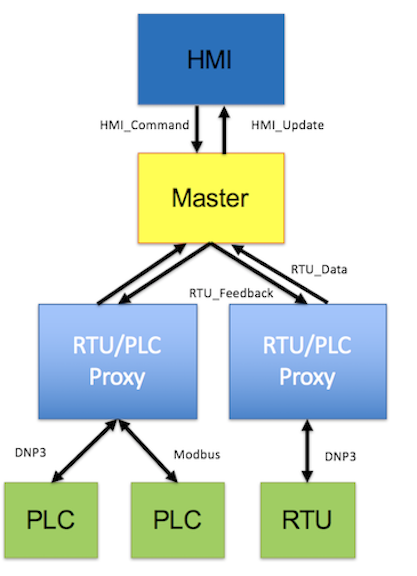
\includegraphics{new_architecture}
  \caption{New Open Source Event Based Architecture}
  \label{fig:2}
  \end{center}
\end{figure}

\indent \indent
The architecture of the entire system is present in figure \ref{fig:2}. The arrows describe
the direction of message flow, with the labels being the type of messages. The system
supports any configuration of proxies and PLCs, with proxies able to support multiple
PLC's of different protocol communication types. 
This configuration is described in the file
\code{config/config.json}. Settings here are used to let all components know about 
the other
elements in the system and allow the system to be configured in a number of ways. 
Information such as the IP address of the PLC's, the communication protocols they use,
and the ports they are listening on are described in this configuration file. 
The system currently supports DNP3 and Modbus, but it is extendable to allow
easy extension to future protocols. The cJSON library is used to support this
functionality \cite{cJSON}\\

\indent
The packet types \code{HMI\_Command}, \code{HMI\_Update}, \code{RTU\_Feedback},
and \code{RTU\_Data} are described in the file \code{common/scada\_packets.h}.
The PLC Proxy gets data from it's PLC's or RTU's speaking either Modbus or DNP3,
and sends this up to the
master in a \code{RTU\_Data} message whenever there is a change of state.
This message is not in any SCADA
protocol, but contains bundled information about the PLC's that the master
needs. The master processes this, updates it's state, and then sends the
HMI a \code{HMI\_Command} message that has all the information the HMI needs
to visualize the scenario. The HMI processes this to present the viewer with
the monitoring information. If the monitor clicks a button, the HMI 
recognizes this event and sends a \code{HMI\_Command} message to the master.
The master gets this, uses the config file to figure out what proxy to forward
this to, and sends a \code{RTU\_Feedback} message to the proxy. The proxy uses
the config to figure out what PLC to route this message to, and translates
the feedback message into a command message in the given PLC's communication
protocol. \\







\section{pvbrowser HMI}

\begin{figure}[ht]
  \begin{center}
  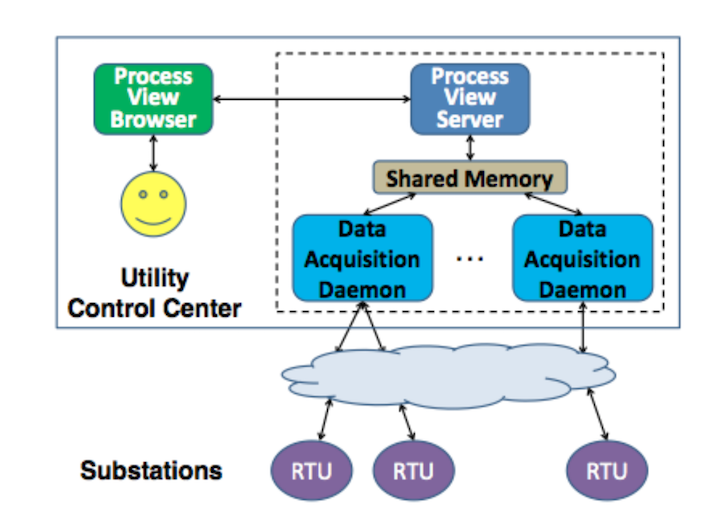
\includegraphics{pvb_architecture}
  \caption{PvBrowser Stock Architecture}
  \label{fig:3}
  \end{center}
\end{figure}

\indent \indent
We use pvbrowser (\cite{pvbrowser}) as our HMI. pvbrowser is an open source SCADA 
software suite. It is used to manage real SCADA deployments, such as the Romanian power
grid. It is a full SCADA solution - it provides an HMI and a master with Modbus
data acquisition daemons that can communicate with RTU's. It's architecture is pictured
in \ref{fig:3}. Early work made it clear that replicating pvbrowser has some of the
same difficulties Kirsch ran into in \cite{Survivable SCADA Via Intrusion-Tolerant Replication}
, but the software had a lot of great components, such as the HMI  and Modbus
communication, that we wished to keep. We changed pvbrowser so that the
Process View Browser Component and Process View Server component where colocated on
the same machine - this is now the HMI box. We then removed the shared memory and
data acquisition daemons, and replaced them with a thread that communicates with the
master, and supplies the pvbrowser thread with the most up to date information of
how to visualize the system. When there is a button click, the pvbrowser thread
sends a message to the master. \\

\indent 
This code is located in \code{hmi}. \code{hmi/master\_exec.cpp} contains the thread
that reads from the master and update's the pvbrowser data structures.
\code{hmi/mask1\_slots.h} contains the code both to visualize the HMI based on the
current data structures, as well as the code to send \code{HMI\_Command} messages
when buttons are clicked. \\

\section{Master}

\indent \indent
The SCADA master is built from scratch in C. It is located in \code{master/scada\_master.c}
and it's data structures are in \code{master/structs.h}. The master uses the config file
to figure out what RTU's or PLC's to route requests to. The master server runs a switch
statement waiting for different message types. When it receives a \code{HMI\_Command}
message, it calls the \code{read\_from\_hmi} method which discovers what the corresponding
\code{RTU\_Feedback} message
should be doing (what field of a RTU it will be modifying) and where to route it,
and then sends it to the proxy. When it recieves a \code{RTU\_Data} message, it updates
it's data structures, then calls the \code{process} method. This method is unique
to each individual scenario. Afterwards it will craft a \code{HMI\_Update} message
and send it to the HMI. \\

\section{Proxy}
\begin{figure}[ht]
  \begin{center}
  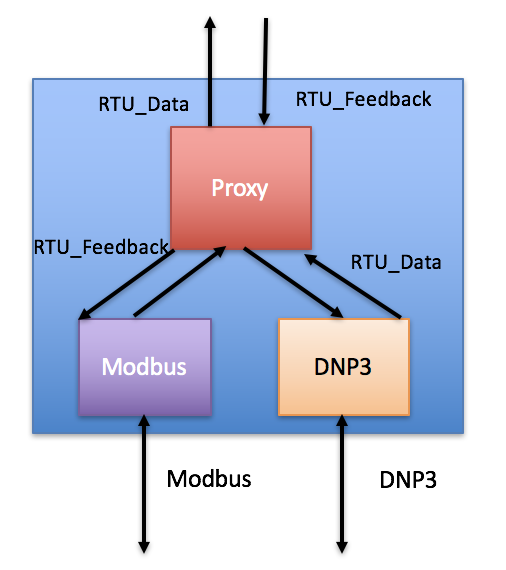
\includegraphics{proxy}
  \caption{Proxy Architecture}
  \label{fig:4}
  \end{center}
\end{figure}

\indent \indent
The architecture of the PLC Proxy is shown in figure \ref{fig:4}. The Proxy
process is located in \code{proxy/proxy.c}. When it runs, it checks it's config
file to see what PLC's or RTU's it's responsible for, and what processes they run.
If there are any PLC's that speak Modbus, it spawns the process 
\code{modbus/modbus\_master}. If it is responsible for any PLC's that speak DNP3 it spawns
the process \code{dnp3/dnp3\_master}. It is set up that if there are any more protocols
implemented, it would spawn their master as well. The master processes are designed
such that they can handle multiple PLC's of the same protocol. For example, if the
proxy is responsible for three PLC's that speak Modbus, it will only spawn one Modbus
 master process.A IPC channel is created for each of the 
child data acquisition daemons such that the proxy can communicate to the child and the
child can communicate with the proxy. When the proxy gets an \code{RTU\_Feedback} message,
it checks to see what protocol the destined PLC speaks, and forwards the 
\code{RTU\_Feedback} message to the designated daemon. When it receives \code{RTU\_Data}
messages from its children, it forwards those messages to the SCADA master. \\

\indent
The Modbus process is a modified version of pvbrowser's Modbus data acquisition daemon
from pvbaddons \cite{pvbaddons}.
It's code is located at \code{modbus/modbus\_master.cpp}. It reads the config file and uses
the information there to figure out where the PLC's that it is responsible for are
located on the network. It then creates TCP connections with them and starts
the <odbus polling protocol. Every time out it polls the PLC's at the location
specified in the config file, and then forwards a \code{RTU\_Data} message with
the corresponding information to the proxy over IPC. If the Modbus master recieves
a \code{RTU\_Feedback} message, it will translate this into the proper Modbus
control message and forward this to the corresponding PLC. \\

\indent
The DNP3 master process uses the OpenDNP3 library (\cite{OpenDNP3}) to implement 
DNP3 communication with it's devices. DNP3 is a more advanced event based communication
protocol that is common in power grid networks. OpenDNP3 provides a modern, C++11 
programming API for implementing DNP3 communication. The code for the DNP3 daemon is in
\code{dnp3/}. The file \code{dnp3/main.cpp} is responsible for reading the config file
and recognizing what PLC's it has to communicate with, and starting a DNP3 session with 
those PLC's. It sets up call-back's for these PLC's, such that when they send an event
update, the code in \code{dnp3/callback.cpp} runs, and creates a \code{RTU\_Data}
message to be sent to the proxy process. The main thread also sets up IPC communication
with the proxy such that when it gets a \code{RTU\_Feedback} message it translates
this into a DNP3 control message and sends it along to the corresponding PLC. \\


\section{Open PLC}

\indent \indent 
We use OpenPLC \cite{OpenPLC} to emulate PLC's and RTU's. It is very useful, as
it allows us to emulate realistic PLC's that a SCADA system would have to
control and monitor. In addition to emulation, OpenPLC software can be deployed to 
many hobby PLC boards to actually control devices. \\

\indent 
OpenPLC is configured by creating a Ladder Logic (LD) or Structured Text (ST) 
description of the PLC. Variables
can be mapped to register positions on the PLC, and manipulated with the
Ladder Logic or Structured Text. These same registers map to Modbus registers. Devices
can then communicate with the Open PLC via Modbus by polling for the desired registers. 
we extended OpenPLC to also map the registers to DNP3 addresses and communicate with 
masters via DNP3. This is done with OpenDNP3, and allows to emulate a wider gambit
of devices.\\

\chapter{Case Study: Power Distribution Scenario}

\section{Overview}

\indent \indent
To demonstrate this architecture used in a real SCADA system we built a Power Distribution
scenario. The scenario is designed with ten PLC's providing the system with power switching
information. An operator can see this, and use it to route power around different
substation.\\

\section{HMI}
\begin{figure}[ht]
  \begin{center}
  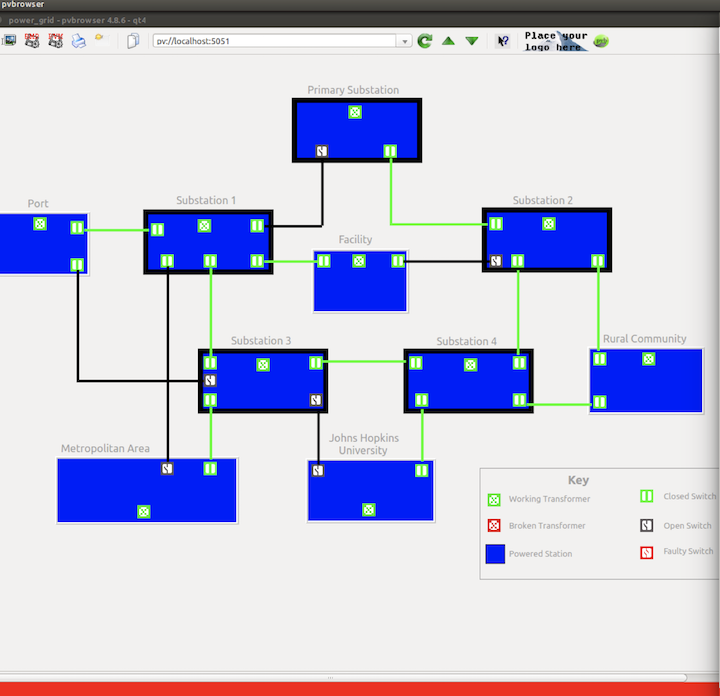
\includegraphics{pvb}
  \caption{pvbrowser HMI}
  \label{fig:5}
  \end{center}
\end{figure}

\indent \indent
The HMI is pictured in figure \ref{fig:5}. The boxes are substations - if they are
blue there is power located at the substation. Power is generated at the
primary substation. If a substation is black than that
substation has no power. The 'x' in the middle of a substation is a transformer. 
If it is red, then
no power can be distributed from that particular substation. If switches are green,
they are closed, if they are black they are open, and if they are red they are tripped,
which means they are broken and can't be modified before they are fixed. When switches
are open or tripped, power can not flow through a line and thus it is black. When switches
are both closed, and one of the substations has power, then power will flow
through the line and it will be green. \\

\indent
To make changes to the system, the operator can click on either the transformers,
or the switches, and the click will cause the system to change
that PLC's state. \\


\section{Master}

\indent \indent

The SCADA master for this scenario runs a version of Breadth First Search to determine
what substations are powered, and what lines are carrying electricity. It does this because
it knows from the PLC's only which switches are open or closed, and which transformers are
on or off. Only the primary substation is known to be powered, and the rest of the 
information for the operator has to be extrapolated from the data the PLC's are providing.
It takes the result of this process, puts it in an array, and sends it to the HMI in a 
\code{HMI\_Update} message.
\\

\indent
The master is able to translate \code{HMI\_Command} messages, which come from the HMI and 
specify what item has been pressed, into \code{RTU\_Feedback} messages, that are tagged to 
a specific PLC and Proxy, and, if the item pressed is a switch, contain the specific
register number the switch should correspond to. \\

\section{Proxy}

\indent \indent
In this system setup there is a proxy for each PLC, so a total of 10 proxies are run.
This is because each PLC is supposed to be located at a different location. \\

\indent
The proxies protocol daemons knows how to translate a \code{RTU\_Feedback} message
into a corresponding Modbus or DNP3 message to send to the PLC or RTU. For DNP3,
switch controls are Analog Output Commands and the transformers are CROB 
instructions. For Modbus, the switch controls send a set register command and
the transformers are force coil commands. 

\section{PLC Emulation}

\begin{figure}[ht]
  \begin{center}
  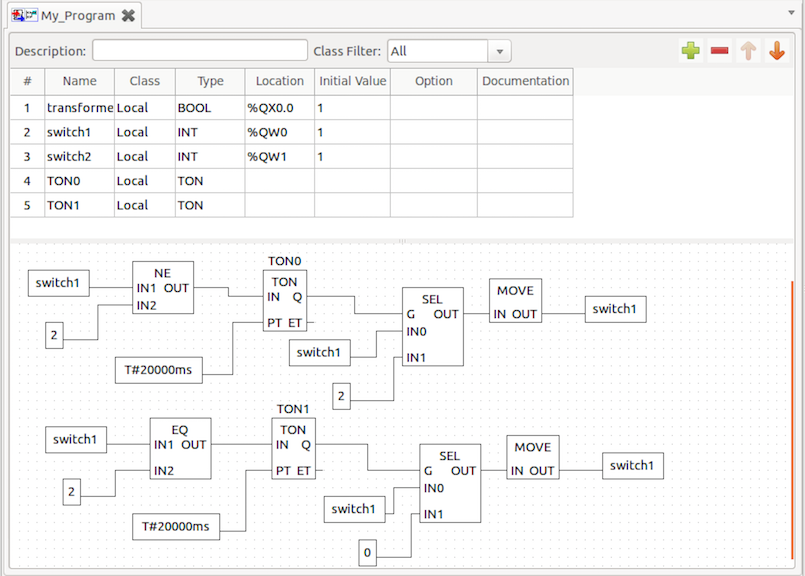
\includegraphics{open_plc}
  \caption{Ladder Logic for RTU 0 in Open PLC}
  \label{fig:6}
  \end{center}
\end{figure}

\indent \indent
To run this scenario we emulated 10 PLC's - one for each substation. The first
three PLC's are emulated with OpenPLC using DNP3. The next two PLC's are emulated with
OpenPLC using Modbus. To demonstrate our system's backwards compatibility, we also emulate
five PLC's with the ASE Test Set 2000 Device \cite{ASE Test Set 2000}. It can emulate
Modbus or DNP3 RTU's and is used by Siemens to test their SCADA equipment. The next three
PLCs are emulated with the ASE device through DNP3, and the last two are emulated
with the ASE device through Modbus. \\

\indent
The PLC's contain data for the transformers and switches. A switch value of 0 is open,
1 is closed, and 2 is tripped. A transformer value of 1 is on and 0 is off.
This data is represented in
two different ways depending on if the device is Modbus or DNP3. If the device is 
Modbus, the transformer is a coil status at register zero, and the switches are 
holding registers at the register it's switch number should be (if a substation
has three switches it will have holding registers at 0, 1, 2 to store that switch's 
data). For DNP3, the registers for the transformers and switches are at the same location
, but instead of Coil Status and Holding Registers it is Binary Output Status
and Analog Output Status. \\

\indent
In this scenario, PLC 0 (the primary substation) has been written with Ladder Logic
in Open PLC. The associated LD program is shown in figure \ref{fig:6}. This program
trips the first switch every 20 seconds, and then un=trips it and sets the status
to open every other 20 seconds. \\


\appendix



\bibliographystyle{unsrt}
\bibliography{sample}

\end{document}

